%\documentclass[handout]{beamer} % \pause disabled
\documentclass[t]{beamer} % \pause enabled
%%%%%%%%%%%%%%%%% Arya's
\usepackage{color,hyperref}
\hypersetup{colorlinks,breaklinks,linkcolor=darkblue,urlcolor=darkblue, anchorcolor=darkblue,citecolor=darkblue}
\usepackage{amsmath}
\usepackage{amsfonts}
\usepackage{amssymb}
\usepackage{mathtools}
\usepackage{enumerate}
\definecolor{darkgreen}{rgb}{0,0.55,0}
\definecolor{orange}{rgb}{1,0.55,0}
\definecolor{darkblue}{rgb}{0.0,0.0,0.5}
\def\Arya#1{{\textcolor{darkgreen}{Arya note: #1}}}

\newtheorem{Thm}{Theorem}


\newcommand{\dataset}{{\cal D}}
\newcommand{\fracpartial}[2]{\frac{\partial #1}{\partial  #2}}
\newcommand{\phibp}{\phi_{ \hspace{-0.025in}\scalebox{.45}{\text{ BP}}}}
\newcommand{\phics}{\phi_{ \hspace{-0.025in}\scalebox{.45}{\text{ CS}}}}
\newcommand{\lone}{$\ell_1$-norm }
%\def\lll{\mbox{\ell_1}}

%%%%%%%%%%%%%%%%% Anima Anandkumar's macros
\DeclareMathOperator{\tw}{tw}
\DeclareMathOperator{\local}{local}
\DeclareMathOperator{\range}{range}
\DeclareMathOperator{\Path}{Path}
\DeclareMathOperator{\Sg}{Sg}
\DeclareMathOperator{\spt}{SP}
\DeclareMathOperator{\avg}{avg}
\DeclareMathOperator{\nbd}{\mathcal{N}}
\DeclareMathOperator{\parent}{Pa}
\DeclareMathOperator{\Cq}{Cq}
\DeclareMathOperator{\TW}{TW}
\DeclareMathOperator{\approxML}{ApproxML}
\DeclareMathOperator{\Bethe}{Bethe}
\DeclareMathOperator{\TRW}{TRW}
\DeclareMathOperator{\conv}{Conv}
\DeclareMathOperator{\dir}{Dir}
\DeclareMathOperator{\mult}{Mult}
\DeclareMathOperator{\cat}{Cat}
\DeclareMathOperator{\crp}{CRP(\gamma)}
\DeclareMathOperator{\ncrp}{nCRP}
\DeclareMathOperator{\node}{node}
\DeclareMathOperator{\nodes}{nodes}
\DeclareMathOperator{\pr}{Pr}
\DeclareMathOperator{\dom}{\bf Dom}
\DeclareMathOperator{\lbp}{LBP}
\DeclareMathOperator{\Corr}{Corr}
\DeclareMathOperator{\hCorr}{\widehat{Corr}}
\DeclareMathOperator{\hSc}{\widehat{\mathcal{S}}}
\DeclareMathOperator{\tr}{Tr}
\DeclareMathOperator{\mst}{MST}
\DeclareMathOperator{\supp}{Supp}
\DeclareMathOperator{\dtv}{d_{TV}}
\DeclareMathOperator{\hdtv}{\hd_{TV}}
\DeclareMathOperator*{\argmin}{arg\,min}
\DeclareMathOperator*{\argmax}{arg\,max}
\DeclareMathOperator*{\esssup}{ess\,sup}
\DeclareMathOperator*{\essinf}{ess\,inf}
\DeclareMathOperator{\dist}{dist}
\DeclareMathOperator{\rank}{Rank}
\DeclareMathOperator{\Krank}{Rank_K}
\DeclareMathOperator{\Det}{Det}
\DeclareMathOperator{\poiss}{Poiss}
\DeclareMathOperator{\unif}{Unif} \DeclareMathOperator{\Deg}{Deg}
\def\simiid{{\overset{i.i.d.}{\sim}}}
\def\lcv{{\,\,\underset{cv}{\leq}\,\,}}
\def\gcv{{\,\,\underset{cv}{\geq}\,\,}}
\def\lcx{{\,\,\underset{cx}{\leq}\,\,}}
\def\gcx{{\,\,\underset{cx}{\geq}\,\,}}
\def\leqst{{\,\,\overset{st}{\leq}\,\,}}
\def\geqst{{\,\,\overset{st}{\geq}\,\,}}
\def\eqdist{{\,\,\overset{d}{=}\,\,}}
\def\geqrh{{\,\,\overset{rh}{\geq}\,\,}}
\def\geqlr{{\,\,\overset{lr}{\geq}\,\,}}
\def\eqlr{{\,\,\overset{lr}{=}\,\,}}
\def\comment{{\mbox{\bf Comment\_Anima: }}}
\def\tha{{\mbox{\tiny th}}}

\DeclareMathOperator{\Aug}{Aug}
\DeclareMathOperator{\watts}{Watts}
\DeclareMathOperator{\girth}{Girth}
\DeclareMathOperator{\PL}{PL}
\DeclareMathOperator{\LP}{LP}
\DeclareMathOperator{\ER}{ER}
\DeclareMathOperator{\reg}{Reg}
\DeclareMathOperator{\Var}{Var}
\DeclareMathOperator{\hSigma}{\widehat{\Sigma}}
\DeclareMathOperator{\Cov}{Cov}
\DeclareMathOperator{\Poiss}{Poiss}
\DeclareMathOperator{\Diag}{Diag}
\DeclareMathOperator{\Diam}{Diam}
\def\erf{\mbox{erf}}
\def\erfc{\mbox{erfc}}
\def\qfunc{\mbox{Q}}
%\def\myexp{\mbox{e}}
\def\snr{\mbox{{SNR}}}
\def\signum{\mbox{sgn}}
\def\Card{\mbox{Card}}
\DeclareMathOperator*{\plim}{plim}
\def\convd{\overset{d}\rightarrow}
\def\convp{\overset{p}\rightarrow}
\newcommand\indep{\protect\mathpalette{\protect\independenT}{\perp}}
\def\independenT#1#2{\mathrel{\rlap{$#1#2$}\mkern2mu{#1#2}}}
\def\pl{{\parallel}}
\DeclarePairedDelimiter\norm{\lVert}{\rVert}
\DeclarePairedDelimiter\nuclearnorm{\lVert}{\rVert_*}
\DeclarePairedDelimiter\onenorm{\lVert}{\rVert_1}
\DeclarePairedDelimiter\znorm{\lVert}{\rVert_0}
\def\rinfnorm{\rVert_{\infty}}
\DeclarePairedDelimiter\infnorm{\lVert}{\rinfnorm}
\def\lnorm{{\lvert\!\lvert\!\lvert}}
\def\rnorm{{\rvert\!\rvert\!\rvert}}
\DeclarePairedDelimiter\gennorm{\lnorm}{\rnorm}
 \DeclarePairedDelimiter\abs{\lvert}{\rvert}
 \DeclarePairedDelimiter\geninfnorm{\lnorm}{\rnorm_{\infty}}
 \DeclarePairedDelimiter\genonenorm{\lnorm}{\rnorm_{1}}
\DeclareMathOperator{\atanh}{atanh}
 \DeclareMathOperator{\sech}{sech}
 \def\0{{\bf 0}}

\DeclareMathOperator{\lea}{\overset{(a)}{\leq}}
\DeclareMathOperator{\leb}{\overset{(b)}{\leq}}
\DeclareMathOperator{\lec}{\overset{(c)}{\leq}}
\DeclareMathOperator{\led}{\overset{(d)}{\leq}}
\DeclareMathOperator{\lee}{\overset{(e)}{\leq}}

\DeclareMathOperator{\eqa}{\overset{(a)}{=}}
\DeclareMathOperator{\eqb}{\overset{(b)}{=}}
\DeclareMathOperator{\eqc}{\overset{(c)}{=}}
\DeclareMathOperator{\eqd}{\overset{(d)}{=}}
\DeclareMathOperator{\eqe}{\overset{(e)}{=}}

\DeclareMathOperator{\gea}{\overset{(a)}{\geq}}
\DeclareMathOperator{\geb}{\overset{(b)}{\geq}}
\DeclareMathOperator{\gec}{\overset{(c)}{\geq}}
\DeclareMathOperator{\ged}{\overset{(d)}{\geq}}
\DeclareMathOperator{\gee}{\overset{(e)}{\geq}}

\def\viz{{viz.,\ \/}}
\def\ie{{i.e.,\ \/}}
\def\eg{{e.g.,\ \/}}
\def\etc{{etc.  }}
\def\ifff{{iff  }}
\def\as{{a.s.  }}
\def\st{{s.t.  }}
\def\wpone{{w.p.}\,1\,\,}
\def\wpp{{w.p.p.}\,\,}
\def\for{\,\,\mbox{for}\quad}
\def\ifmbox{\,\,\mbox{if}\quad}
\def\nn{\nonumber}
%\def\qed{\hfill$\Box$}

\def\qed{\hfill\hbox{${\vcenter{\vbox{
    \hrule height 0.4pt\hbox{\vrule width 0.4pt height 6pt
    \kern5pt\vrule width 0.4pt}\hrule height 0.4pt}}}$}}
\def\complx{\mathbb{C}}

%%%%%%%%%%%%%%%%%%%%%%%%%%%%%%%%%%%%%%%%%%%%%%%%%%%%%%%%%%%%% Color

\def\tcr{\textcolor{red}}
\def\tcb{\textcolor{blue}}
\def\tcg{\textcolor{green}}
\def\tcw{\textcolor{white}}
\def\tcm{\textcolor{magenta}}
\def\tccyan{\textcolor{cyan}}
\def\tcv{\textcolor{violet}}
\definecolor{myred}{rgb}{0.3,0.0,0.7}
\definecolor{dkg}{rgb}{0.1,0.7,0.2}
\definecolor{dkb}{rgb}{0.0,0.2,0.8}

\def\tcdkb{\textcolor{dkb}}
\def\tcdkg{\textcolor{dkg}}


%%%%%%%%%%%%%%%%%%%%%%%%%%%%%%%%%%%%%%%%%%%%%%%%%%%%%%%%%%%%%
\newcommand{\Amsc}{\mathscr{A}}
\newcommand{\Cmsc}{\mathscr{C}}
\newcommand{\Dmsc}{\mathscr{D}}
\newcommand{\Emsc}{\mathscr{E}}
\newcommand{\Fmsc}{\mathscr{F}}
\newcommand{\Gmsc}{\mathscr{G}}
\newcommand{\Hmsc}{\mathscr{H}}
\newcommand{\Kmsc}{\mathscr{K}}
\newcommand{\Nmsc}{\mathscr{N}}
\newcommand{\Pmsc}{\mathscr{P}}
\newcommand{\Qmsc}{\mathscr{Q}}
\newcommand{\Rmsc}{\mathscr{R}}
\newcommand{\Smsc}{\mathscr{S}}
\newcommand{\Tmsc}{\mathscr{T}}
\newcommand{\Umsc}{\mathscr{U}}
\newcommand{\Xmsc}{\mathscr{X}}
\newcommand{\Ymsc}{\mathscr{Y}}

%%%%%%%%%%%%%%%%%%%%%%%%%%%%%%%%%%%%%%%%%%%%%%%%%%%%%%%%%%%%% Hat
\def\ha{\widehat{a}}
\def\hb{\widehat{b}}
\def\hc{\widehat{c}}
\def\hd{\widehat{d}}
\def\he{\widehat{e}}
\def\hf{\widehat{f}}
\def\hg{\widehat{g}}
\def\hh{\widehat{h}}
\def\hi{\widehat{i}}
\def\hj{\widehat{j}}
\def\hk{\widehat{k}}
\def\hl{\widehat{l}}
\def\hm{\widehat{m}}
\def\hn{\widehat{n}}
\def\ho{\widehat{o}}
\def\hp{\widehat{p}}
\def\hq{\widehat{q}}
\def\hr{\widehat{r}}
\def\hs{\widehat{s}}
\def\hatt{\widehat{t}}
\def\hu{\widehat{u}}
\def\hv{\widehat{v}}
\def\hw{\widehat{w}}
\def\hx{\widehat{x}}
\def\hy{\widehat{y}}
\def\hz{\widehat{z}}

\def\hA{\widehat{A}}
\def\hB{\widehat{B}}
\def\hC{\widehat{C}}
\def\hD{\widehat{D}}
\def\hE{\widehat{E}}
\def\hF{\widehat{F}}
\def\hG{\widehat{G}}
\def\hH{\widehat{H}}
\def\hI{\widehat{I}}
\def\hJ{\widehat{J}}
\def\hK{\widehat{K}}
\def\hL{\widehat{L}}
\def\hM{\widehat{M}}
\def\hN{\widehat{N}}
\def\hO{\widehat{O}}
\def\hP{\widehat{P}}
\def\hQ{\widehat{Q}}
\def\hR{\widehat{R}}
\def\hS{\widehat{S}}
\def\hT{\widehat{T}}
\def\hU{\widehat{U}}
\def\hV{\widehat{V}}
\def\hW{\widehat{W}}
\def\hX{\widehat{X}}
\def\hY{\widehat{Y}}
\def\hZ{\widehat{Z}}
\def\hlambda{\widehat{\lambda}}
\def\hpi{\widehat{\pi}}
\def\hnu{\widehat{\nu}}
\def\hbd{\widehat{\mathbf{d}}}
\def\bLambda{\mathbf{\Lambda}}

%%%%%%%%%%%%%%%%%%%%%%%%%%%%%%%%%%%%%%%%%%%%%%%%%%%%%%%%%%%%% Bold
\def\bfnu{{\boldsymbol {\nu}}}
\def\bfzero{{\mathbf{0}}}
\def\bfone{{\mathbf{1}}}
\def\bfa{{\mathbf a}}
\def\bfb{{\mathbf b}}
\def\bfc{{\mathbf c}}
\def\bfd{{\mathbf d}}
\def\bfe{{\mathbf e}}
\def\bff{{\mathbf f}}
\def\bfg{{\mathbf g}}
\def\bfh{{\mathbf h}}
\def\bfi{{\mathbf i}}
\def\bfj{{\mathbf j}}
\def\bfk{{\mathbf k}}
\def\bfl{{\mathbf l}}
\def\bfm{{\mathbf m}}
\def\bfn{{\mathbf n}}
\def\bfo{{\mathbf o}}
\def\bfp{{\mathbf p}}
\def\bfq{{\mathbf q}}
\def\bfr{{\mathbf r}}
\def\bfs{{\mathbf s}}
\def\bft{{\mathbf t}}
\def\bfu{{\mathbf u}}
\def\bfv{{\mathbf v}}
\def\bfw{{\mathbf w}}
\def\bfx{{\mathbf x}}
\def\bfy{{\mathbf y}}
\def\bfz{{\mathbf z}}

\def\bfA{{\mathbf A}}
\def\bfB{{\mathbf B}}
\def\bfC{{\mathbf C}}
\def\bfD{{\mathbf D}}
\def\bfE{{\mathbf E}}
\def\bfF{{\mathbf F}}
\def\bfG{{\mathbf G}}
\def\bfH{{\mathbf H}}
\def\bfI{{\mathbf I}}
\def\bfJ{{\mathbf J}}
\def\bfK{{\mathbf K}}
\def\bfL{{\mathbf L}}
\def\bfM{{\mathbf M}}
\def\bfN{{\mathbf N}}
\def\bfO{{\mathbf O}}
\def\bfP{{\mathbf P}}
\def\bfQ{{\mathbf Q}}
\def\bfR{{\mathbf R}}
\def\bfS{{\mathbf S}}
\def\bfT{{\mathbf T}}
\def\bfU{{\mathbf U}}
\def\bfV{{\mathbf V}}
\def\bfW{{\mathbf W}}
\def\bfX{{\mathbf X}}
\def\bfY{{\mathbf Y}}
\def\bfZ{{\mathbf Z}}


%%%%%%%%%%%%%%%%%%%%%%%%%%%%%%%%%%%%%%%%%%%%%%%%%%%%%%%%%%%%% Bold Symbols
\def\alphabf{\hbox{\boldmath$\alpha$\unboldmath}}
\def\betabf{\hbox{\boldmath$\beta$\unboldmath}}
\def\gammabf{\hbox{\boldmath$\gamma$\unboldmath}}
\def\deltabf{\hbox{\boldmath$\delta$\unboldmath}}
\def\epsilonbf{\hbox{\boldmath$\epsilon$\unboldmath}}
\def\zetabf{\hbox{\boldmath$\zeta$\unboldmath}}
\def\etabf{\hbox{\boldmath$\eta$\unboldmath}}
\def\iotabf{\hbox{\boldmath$\iota$\unboldmath}}
\def\kappabf{\hbox{\boldmath$\kappa$\unboldmath}}
\def\lambdabf{\hbox{\boldmath$\lambda$\unboldmath}}
\def\mubf{\hbox{\boldmath$\mu$\unboldmath}}
\def\nubf{\hbox{\boldmath$\nu$\unboldmath}}
\def\xibf{\hbox{\boldmath$\xi$\unboldmath}}
\def\pibf{\hbox{\boldmath$\pi$\unboldmath}}
\def\rhobf{\hbox{\boldmath$\rho$\unboldmath}}
\def\sigmabf{\hbox{\boldmath$\sigma$\unboldmath}}
\def\taubf{\hbox{\boldmath$\tau$\unboldmath}}
\def\upsilonbf{\hbox{\boldmath$\upsilon$\unboldmath}}
\def\phibf{\hbox{\boldmath$\phi$\unboldmath}}
\def\chibf{\hbox{\boldmath$\chi$\unboldmath}}
\def\psibf{\hbox{\boldmath$\psi$\unboldmath}}
\def\omegabf{\hbox{\boldmath$\omega$\unboldmath}}
\def\inftybf{\hbox{\boldmath$\infty$\unboldmath}}
\def\hSigmabf{\hbox{$\widehat{\bf \Sigma}$}}
\def\Sigmabf{\hbox{$\bf \Sigma$}}
\def\Upsilonbf{\hbox{$\bf \Upsilon$}}
\def\Omegabf{\hbox{$\bf \Omega$}}
\def\Deltabf{\hbox{$\bf \Delta$}}
\def\Gammabf{\hbox{$\bf \Gamma$}}
\def\Thetabf{\hbox{$\bf \Theta$}}
\def\Lambdabf{\mbox{$ \bf \Lambda $}}
\def\Xibf{\hbox{\bf$\Xi$}}
\def\Pibf{{\bf \Pi}}
\def\thetabf{{\mbox{\boldmath$\theta$\unboldmath}}}
\def\Upsilonbf{\hbox{\boldmath$\Upsilon$\unboldmath}}
\newcommand{\Phibf}{\mbox{${\bf \Phi}$}}
\newcommand{\Psibf}{\mbox{${\bf \Psi}$}}
\def\olambda{\mathfrak{o}(\lambda)}
\def\complex{\mathfrak{C}}

%%%%%%%%%%%%%%%%%%%%%%%%%%%%%%%%%%%%%%%%%%%%%%%%%%%%%%%%%%%%% Bar
\def\brzero{{\overline{{0}}}}
\def\brone{{\overline{{1}}}}
\def\bra{{\overline{a}}}
\def\brb{{\overline{b}}}
\def\brc{{\overline{c}}}
\def\brd{{\overline{d}}}
\def\bre{{\overline{e}}}
\def\brf{{\overline{f}}}
\def\brg{{\overline{g}}}
\def\brh{{\overline{h}}}
\def\bri{{\overline{i}}}
\def\brj{{\overline{j}}}
\def\brk{{\overline{k}}}
\def\brl{{\overline{l}}}
\def\brm{{\overline{m}}}
\def\brn{{\overline{n}}}
\def\bro{{\overline{o}}}
\def\brp{{\overline{p}}}
\def\brq{{\overline{q}}}
\def\brr{{\overline{r}}}
\def\brs{{\overline{s}}}
\def\brt{{\overline{t}}}
\def\bru{{\overline{u}}}
\def\brv{{\overline{v}}}
\def\brw{{\overline{w}}}
\def\brx{{\overline{x}}}
\def\bry{{\overline{y}}}
\def\brz{{\overline{z}}}

\def\brA{{\overline{A}}}
\def\brB{{\overline{B}}}
\def\brC{{\overline{C}}}
\def\brD{{\overline{D}}}
\def\brE{{\overline{E}}}
\def\brF{{\overline{F}}}
\def\brG{{\overline{G}}}
\def\brH{{\overline{H}}}
\def\brI{{\overline{I}}}
\def\brJ{{\overline{J}}}
\def\brK{{\overline{K}}}
\def\brL{{\overline{L}}}
\def\brM{{\overline{M}}}
\def\brN{{\overline{N}}}
\def\brO{{\overline{O}}}
\def\brP{{\overline{P}}}
\def\brQ{{\overline{Q}}}
\def\brR{{\overline{R}}}
\def\brS{{\overline{S}}}
\def\brT{{\overline{T}}}
\def\brU{{\overline{U}}}
\def\brV{{\overline{V}}}
\def\brW{{\overline{W}}}
\def\brX{{\overline{X}}}
\def\brY{{\overline{Y}}}
\def\beZ{{\overline{Z}}}


%%%%%%%%%%%%%%%%%%%%%%%%%%%%%%%%%%%%%%%%%%%%%%%%%%%%%%%%%%%%% Bar Bold 
\def\bbfzero{{\overline{\mathbf{0}}}}
\def\bbfone{{\overline{\mathbf{1}}}}
\def\bbfa{{\overline{\mathbf a}}}
\def\bbfb{{\overline{\mathbf b}}}
\def\bbfc{{\overline{\mathbf c}}}
\def\bbfd{{\overline{\mathbf d}}}
\def\bbfe{{\overline{\mathbf e}}}
\def\bbff{{\overline{\mathbf f}}}
\def\bbfg{{\overline{\mathbf g}}}
\def\bbfh{{\overline{\mathbf h}}}
\def\bbfi{{\overline{\mathbf i}}}
\def\bbfj{{\overline{\mathbf j}}}
\def\bbfk{{\overline{\mathbf k}}}
\def\bbfl{{\overline{\mathbf l}}}
\def\bbfm{{\overline{\mathbf m}}}
\def\bbfn{{\overline{\mathbf n}}}
\def\bbfo{{\overline{\mathbf o}}}
\def\bbfp{{\overline{\mathbf p}}}
\def\bbfq{{\overline{\mathbf q}}}
\def\bbfr{{\overline{\mathbf r}}}
\def\bbfs{{\overline{\mathbf s}}}
\def\bbft{{\overline{\mathbf t}}}
\def\bbfu{{\overline{\mathbf u}}}
\def\bbfv{{\overline{\mathbf v}}}
\def\bbfw{{\overline{\mathbf w}}}
\def\bbfx{{\overline{\mathbf x}}}
\def\bbfy{{\overline{\mathbf y}}}
\def\bbfz{{\overline{\mathbf z}}}

\def\bbfA{{\overline{\mathbf A}}}
\def\bbfB{{\overline{\mathbf B}}}
\def\bbfC{{\overline{\mathbf{C}}}}
\def\bbfD{{\overline{\mathbf D}}}
\def\bbfE{{\overline{\mathbf E}}}
\def\bbfF{{\overline{\mathbf F}}}
\def\bbfG{{\overline{\mathbf G}}}
\def\bbfH{{\overline{\mathbf H}}}
\def\bbfI{{\overline{\mathbf I}}}
\def\bbfJ{{\overline{\mathbf J}}}
\def\bbfK{{\overline{\mathbf K}}}
\def\bbfL{{\overline{\mathbf L}}}
\def\bbfM{{\overline{\mathbf M}}}
\def\bbfN{{\overline{\mathbf N}}}
\def\bbfO{{\overline{\mathbf O}}}
\def\bbfP{{\overline{\mathbf P}}}
\def\bbfQ{{\overline{\mathbf Q}}}
\def\bbfR{{\overline{\mathbf R}}}
\def\bbfS{{\overline{\mathbf S}}}
\def\bbfT{{\overline{\mathbf T}}}
\def\bbfU{{\overline{\mathbf U}}}
\def\bbfV{{\overline{\mathbf V}}}
\def\bbfW{{\overline{\mathbf W}}}
\def\bbfX{{\overline{\mathbf X}}}
\def\bbfY{{\overline{\mathbf Y}}}
\def\bbfZ{{\overline{\mathbf Z}}}

%%%%%%%%%%%%%%%%%%%%%%%%%%%%%%%%%%%%%%%%%%%%%%%%%%%%%%%%%%%%% Calligraphic
\def\Ac{{\cal A}}
\def\Bc{{\cal B}}
\def\Cc{{\cal C}}
\def\Dc{{\cal D}}
\def\Ec{{\cal E}}
\def\Fc{{\cal F}}
\def\Gc{{\cal G}}
\def\Hc{{\cal H}}
\def\Ic{{\cal I}}
\def\Jc{{\cal J}}
\def\Kc{{\cal K}}
\def\Lc{{\cal L}}
\def\Mc{{\cal M}}
\def\Nc{{\cal N}}
\def\Oc{{\cal O}}
\def\Pc{{\cal P}}
\def\Qc{{\cal Q}}
\def\Rc{{\cal R}}
\def\Sc{{\cal S}}
\def\Tc{{\cal T}}
\def\Uc{{\cal U}}
\def\Vc{{\cal V}}
\def\Wc{{\cal W}}
\def\Xc{{\cal X}}
\def\Yc{{\cal Y}}
\def\Zc{{\cal Z}}


%%%%%%%%%%%%%%%%%%%%%%%%%%%%%%%%%%%%%%%%%%%%%%%%%%%%%%%%%%%%% Mathbb

\def\Abb{{\mathbb A}}
\def\BBb{{\mathbb B}}% different
\def\Cbb{{\mathbb C}}
\def\Dbb{{\mathbb D}}
\def\Ebb{{\mathbb E}}
\def\Fbb{{\mathbb F}}
\def\Gbb{{\mathbb G}}
\def\Hbb{{\mathbb H}}
\def\Ibb{{\mathbb I}}
\def\Jbb{{\mathbb J}}
\def\Kbb{{\mathbb K}}
\def\Lbb{{\mathbb L}}
\def\Mbb{{\mathbb M}}
\def\Nbb{{\mathbb N}}
\def\Obb{{\mathbb O}}
\def\Pbb{{\mathbb P}}
\def\Qbb{{\mathbb Q}}
\def\Rbb{{\mathbb R}}
\def\Sbb{{\mathbb S}}
\def\Tbb{{\mathbb T}}
\def\Ubb{{\mathbb U}}
\def\Vbb{{\mathbb V}}
\def\Wbb{{\mathbb W}}
\def\Xbb{{\mathbb X}}
\def\Ybb{{\mathbb Y}}
\def\Zbb{{\mathbb Z}}

%%%%%%%%%%%%%%%%%%%%%%%%%%%%%%%%%%%%%%%%%%%%%%%%%%%%%%%%%%%%% Command Abbreviations
%\newcommand{\bprfof}{\begin{proof_of}}
%\newcommand{\eprfof}{\end{proof_of}}
\newcommand{\bprf}{\begin{proof}}
\newcommand{\eprf}{\end{proof}}
%\newcommand{\bp}{\begin{psfrags}}
%\newcommand{\ep}{\end{psfrags}}
%\newcommand{\bl}{\begin{lemma}}
%\newcommand{\el}{\end{lemma}}
\newcommand{\bt}{\begin{theorem}}
\newcommand{\et}{\end{theorem}}
%\newcommand{\bc}{\begin{center}}
%\newcommand{\ec}{\end{center}}
%\newcommand{\bi}{\begin{itemize}}
%\newcommand{\ei}{\end{itemize}}
%\newcommand{\ben}{\begin{enumerate}}
%\newcommand{\een}{\end{enumerate}}
%\newcommand{\bd}{\begin{definition}}
%\newcommand{\ed}{\end{definition}}
\def\beq{\begin{equation}\begin{aligned}}
\def\eeq{\end{aligned}\end{equation}\noindent}
\def\beqq{\begin{equation*}\begin{aligned}}
\def\eeqq{\end{aligned}\end{equation*}\noindent}
\def\beqn{\begin{eqnarray}}
\def\eeqn{\end{eqnarray} \noindent}
%\def\beqnn{  \begin{eqnarray*}}
%\def\eeqnn{\end{eqnarray*}  \noindent}
%\def\bcase{  \begin{numcases}}
%\def\ecase{\end{numcases}   \noindent}
%\def\bsbcase{  \begin{subnumcases}}
%\def\esbcase{\end{subnumcases}   \noindent}
%
%\def\endproof{\hfill\blacksquare}
%\def\defeq{{:=}}%{{\stackrel{\Delta}{=}}}
%
%

\usepackage{datetime}
\def\vecbold#1{{\boldsymbol#1}}

\newdateformat{monthyeardate}{%
  \monthname[\THEMONTH], \THEYEAR}

\usepackage[linesnumbered,ruled]{algorithm2e}
\usetheme{Madrid}
\setbeamertemplate{footline}
{
  \leavevmode%
  \hbox{%
  \begin{beamercolorbox}[wd=.333333\paperwidth,ht=2.25ex,dp=1ex,center]{author in head/foot}%
    \usebeamerfont{author in head/foot}\insertshortauthor
  \end{beamercolorbox}%
  \begin{beamercolorbox}[wd=.333333\paperwidth,ht=2.25ex,dp=1ex,center]{title in head/foot}%
    \usebeamerfont{title in head/foot}\insertshorttitle
  \end{beamercolorbox}%
  \begin{beamercolorbox}[wd=.333333\paperwidth,ht=2.25ex,dp=1ex,right]{date in head/foot}%
    \usebeamerfont{date in head/foot}\insertshortdate{}\hspace*{2em}
    \insertframenumber{} / \inserttotalframenumber\hspace*{2ex} 
  \end{beamercolorbox}}%
  \vskip0pt%
}
\makeatother
\title{Genomic Time-Series Data Analysis}
\subtitle{}
\author[Arya Iranmehr]
{%
  \texorpdfstring{
      \centering
      Arya Iranmehr\\
      \href{mailto:airanmehr@ucsd.edu}{airanmehr@ucsd.edu}
  }
  {Arya Iranmehr}
}
%\email{}
\institute{
Bafna's Lab\\
University of California, San Diego}
\date{
\monthyeardate\today}
\subject{Optimization}
\usefonttheme{serif} % default family is serif
\AtBeginSection[]
  {
     \begin{frame}<beamer>
     \frametitle{Agenda}
     \tableofcontents[currentsection,currentsubsection]
     \end{frame}
  }
\AtBeginSubsection[]
{
  \begin{frame}<beamer>{Outline}
    \tableofcontents[currentsection,currentsubsection]
  \end{frame}
}

\begin{document}
\begin{frame}
  \titlepage
\end{frame}
\begin{frame}{Outline}
  \tableofcontents
\end{frame}


\section{Introduction}
\subsection{Motivation}
\begin{frame}{Motivation I: Importance of  Genetic adaptation}
\begin{itemize}
\item Genetic adaptation is the central evolutionary process which is at the core of some of the challenges facing humanity
\item The challenge arises from the fact that adversary organism's ability to adapt to drugs. For instance
\begin{itemize}
\item Parasite: Malaria may have killed half of all the people that ever lived\footnote{John Whitfield, Portrait of a serial killer, Nature News, 2002.}.
\item Bacteria: The world, is poised to enter a ‘post-antibiotic’ era\footnote{Antibiotic resistance sweeping developing world, Nature News, 2014.}.
\item Virus: HIV
\item Pests: Crop pests
\item Cancer Tumors
\item etc.
\end{itemize}
\item Identifying genes or regions under selection is the first step to a better drug design.
\end{itemize}
\end{frame}

\begin{frame}{Motivation II: NGS, PoolSeq, HPC}
\begin{itemize}
\item {\bf Data Availability:} Next Generation Sequencing (NGS) has made genomic data available at reasonable cost \emphr{for each individual}.
\pause
\item {\bf Population Statistics:} 
\begin{itemize}
\item Most of population genetics algorithms for analysing adaptation process population Allele Frequency (AF) at each site.
\item To compute AF, typically all the individuals are sequenced separately and the population AF is computed for each site.
\item For model (small) organisms where a single animal does not provide enough DNA, it is more effective to pool them together and then sequence.
\item \emphr{PoolSeq} offers a more cost-effective way of computing AF, by sequencing whole population together and computing AF directly. 
\end{itemize}
\pause
\item {\bf Computational Power:} High Performance Computing (\emphr{HPC}) lets us fit more complicated models such as Nonlinear Least-Squares and Gaussian Processes on larger datasets.
\end{itemize}
\end{frame}

\begin{frame}{Motivation III : (Modern) Experimental Evolution}
\begin{itemize}
\item  Experimental evolution (EE) is a very old tradition in biology, which researchers expose an evolving population to a \emphr{selective pressure}, and study the response in a \emphr{controlled environment} at \emphr{different generations}.
\item Modern EE makes inference based on on molecular data.
\end{itemize}
\end{frame}

\begin{frame}{Motivation IV : Evolve and Re-Sequence Paradigm}
\begin{itemize}
\item  In short,   {\bf EE + PoolSeq = Evolve \& ReSequence (E\&R)}
\item E\&R enables us to analyse \emphr{multiple observations of population statistics} in time instead of one, leading to more accurate prediction and identifying more complex adaptations.
\item E.g., Haddad'd lab \footnote{\tiny Zhou et al., Experimental selection for Drosophila survival in extremely low O2 environment, PLoS One,2007.} evolved flies to adapt to hypoxia for over 300 generations, and identified many genes involved in hypoxia tolerance.
\item E.g., dark pigmentation in response to UV radiation \footnote{\tiny Schlötterer, C., et al. "Combining experimental evolution with next-generation sequencing: a powerful tool to study adaptation from standing genetic variation." Heredity , 2014.}
\end{itemize}
\end{frame}

\begin{frame}
\begin{figure}
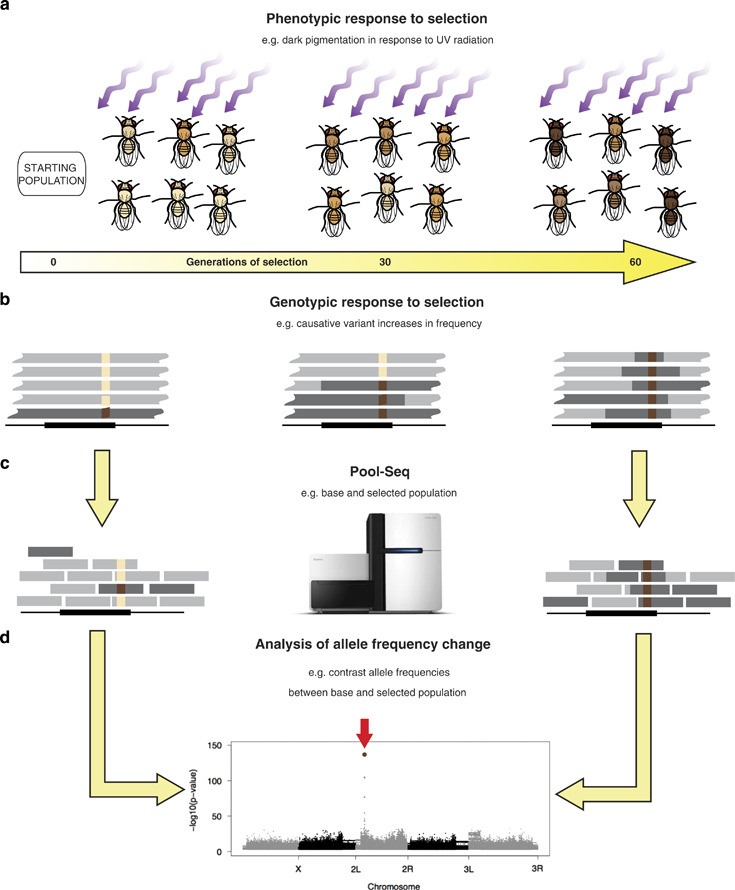
\includegraphics[trim={0 2.1in 0 0},clip, scale=0.65]{eg.jpg} 
\end{figure}

\end{frame}
\subsection{Goal}
\begin{frame}{Goal}
Given Population Statistics (e.g. AF) at different generations (e.g. 10,20,30,40,50) we would like to have a better parametric model for explaining data (Maximum Likelihood) in order to answer

\begin{enumerate}[(i)]
\item Is there a selection happening?
\item If so, where is it?
\item what is the strength of selection?
\item ...
\end{enumerate}
\end{frame}
\subsection{Background}
\begin{frame}{Background}
\begin{itemize}
\item Traditionally, methods for detecting selection  process an snapshot of genome to detect a Selective Sweep.
\item Selective Sweep is rapid expansion of adaptive alleles in populations leading to reduction of polymorphisms.
\item Tajima’s D is the classical test that measures reduction of polymorphisms
\item HKA, LRH, EHH, SFS tests are based on similar objective to detect selection \emphr{after fixation}.
\end{itemize}
\end{frame}
\section{Method}
\subsection{notation}
\begin{frame}{Notation}
\begin{itemize}
\item We consider diploid bi-allelic single-locus Wright-Fisher model with no mutations.
\item At each loci, AFs from generation to generation are described by the random process $\{x_{t}\}$	 for which 
\begin{equation}
x_{t+1} = f(x_t;s,h) + \epsilon_t
\label{eq:trans0} 
\end{equation}
$s$ is selection strength, $h$ is over-dominance and $\epsilon_t \sim \Nc(0,\sigma^2_0)$ is the random noise due to genetic drift and we have
\begin{equation}
  f(x;s,0.5)=x+\frac{sx(1-x)}{2+2sx}\;.
  \label{eq:hequalshalf}
\end{equation}
\item Initial AF at $L$ sites is evolved in $R$ independent replicates and $T$ samples are taken for each replicate, i.e., problem data is $\bfX \in [0,1]^{R \times L \times T}$.
\end{itemize}
\end{frame}
\subsection{Related Work}
\begin{frame}{Gaussian Process \footnote{\tiny Terhorst et. al. "Multi-locus analysis of genomic time series data from experimental evolution." (2015)}}
\begin{itemize}
\item Gaussian Process(GP) is generalization of multivariate Gaussian distribution which assumes any subset of observations are jointly Gaussian.
\item GP is fully determined by mean function $\mu(t;s,x_0)$ and covariance function $\Sigma(t_1,t_2;s,x_0)$.
\item using Mathematica they derived closed form approximation for mean and covariance functions and performed maximum likelihood
\beq
s_\ell^* = \underset{s}{\arg \max} \Lc(s|X_{:,\ell,:})
\eeq
and for each site likelihood ratio is given by
\beq
\Lambda_\ell=\frac{\Lc(s=s_l^*|X_{:,\ell,:})}{\Lc(s=0|X_{:,\ell,:})}
\eeq
\end{itemize}
\end{frame}

\subsection{Proposed Methods}
\begin{frame}{Analysis of transition function}
\begin{itemize}
\item By differentiating update equations ($x_{t+1}=x_t+\frac{sx_t(1-x_t)}{2+2sx_t}$ w.r.t. and solving differential equation, we have
\beq
\nu_t(s)=\frac{1}{1+e^{-st/2+c}}
\eeq
where $c=\log\left(x_0/(1-x_0)\right)$
\end{itemize}
\hspace{-0.6in}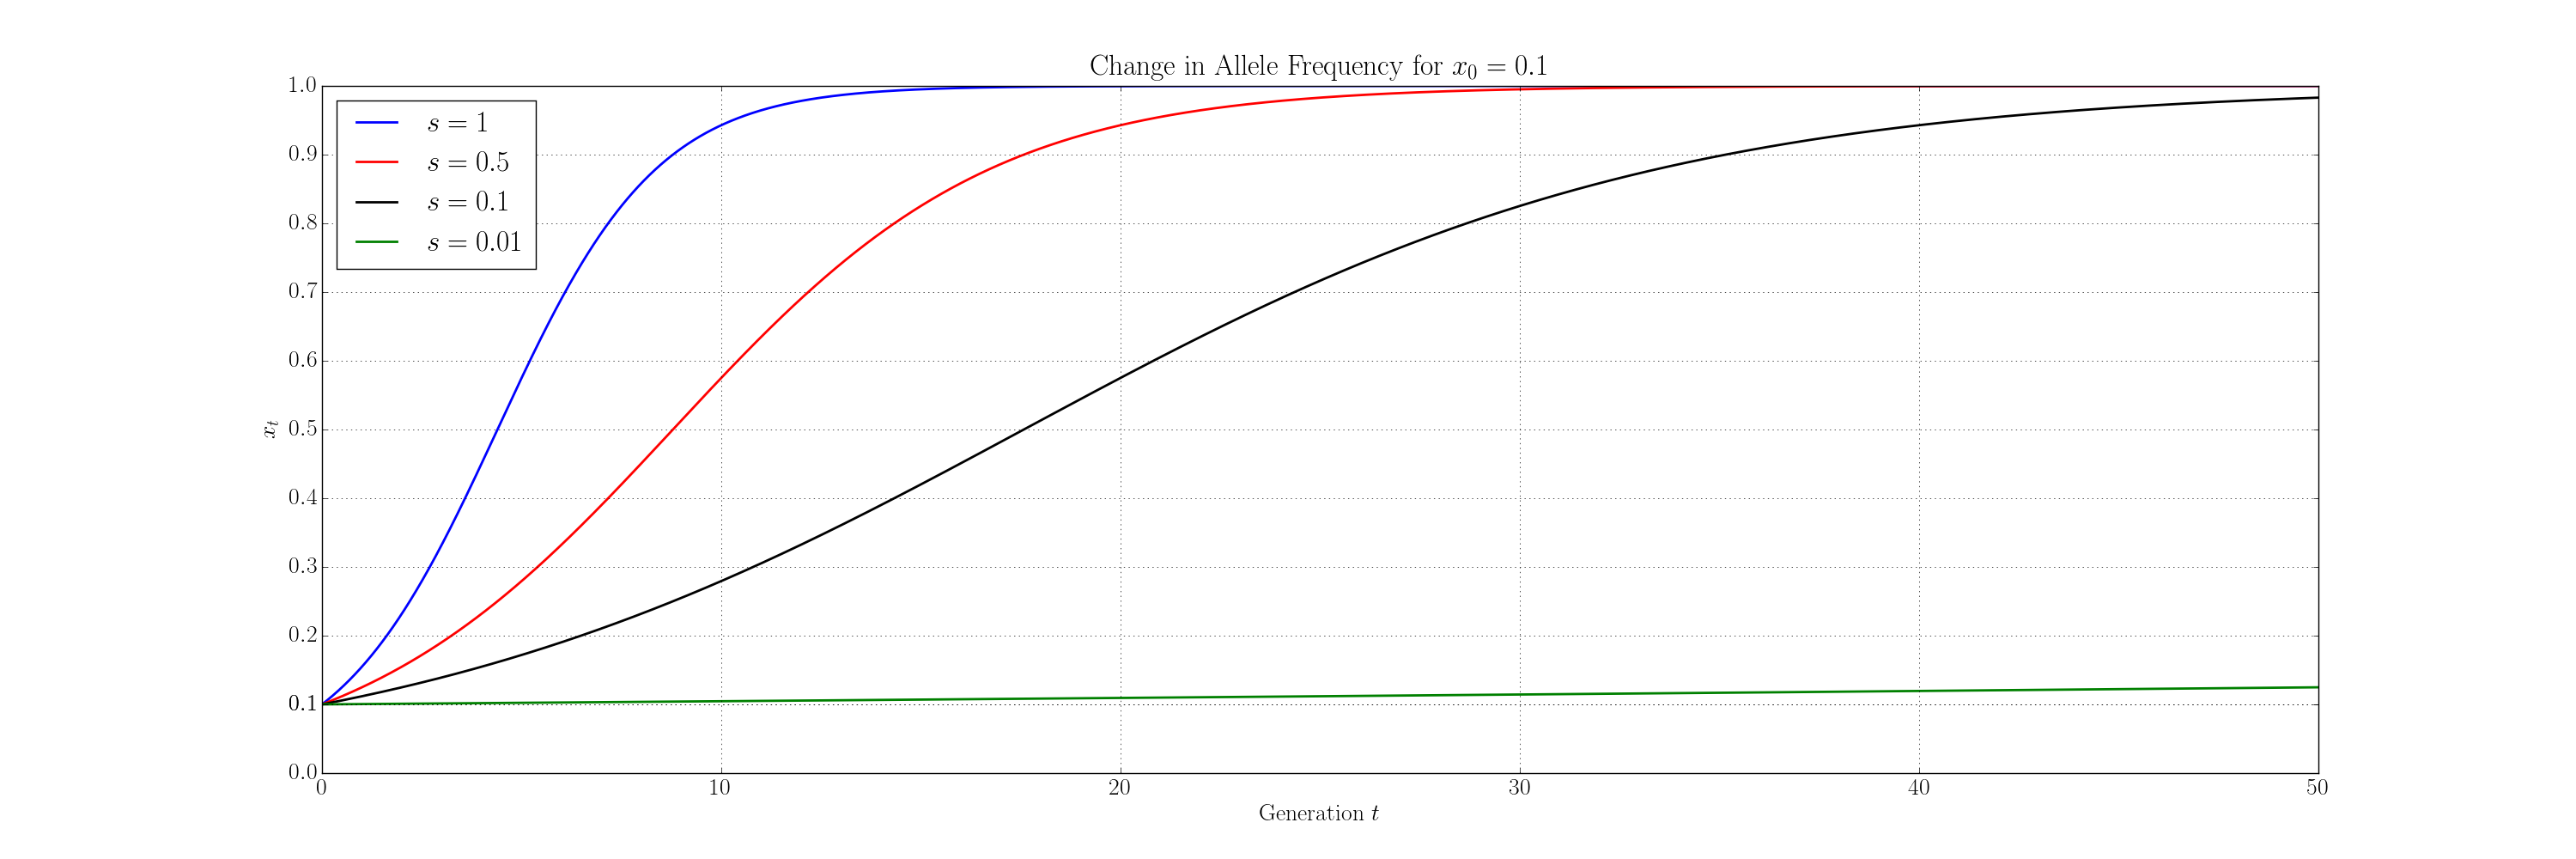
\includegraphics[scale=0.2]{sigmoid}
\end{frame}
\begin{frame}{Naive Method}
\begin{itemize}
\item If we observe $x_t$, we can solve the sigmoid equation for $s$
\begin{equation}
  s^*(t)=\frac{2}{t} \log \left( \frac{x_t(1-x_0)}{x_0 (1-x_t)} \right) 
  \label{eq:naive2point}
\end{equation}
To reduce the variance we can average all the naive estimates for all times 
\begin{equation}
  s^*=\frac{1}{|\Tc|}\sum_{t\in \Tc}\frac{2}{t} \log \left( \frac{x_t
      (1-x_0)}{x_0 (1-x_t)} \right) 
  \label{eq:naive}
\end{equation}
where $\Tc=\{\tau_1,\tau_2,\cdots, \tau_T \}$ is sampling times.
\end{itemize}
\end{frame}
\begin{frame}{Nonlinear Gaussian Model}
\begin{itemize}
\item Assuming genetic drift noise is Gaussian with zero mean and unit variance, we have
\beq
x_t \sim \Nc(\nu_t,1)
\eeq
where by defining 
\[
\vecbold{\nu}(s) = [\nu_{\tau_1}(s),\ldots,\nu_{\tau_T}(s)]
\]
for all $r$ we have $\bfX_{r,l,:}\sim \Nc(\vecbold{\nu},I)$.
\item Finding Maximum Likelihood Estimate of the nonlinear Gaussian model amounts to solve the nonlinear least-squares problem
\begin{equation}
  s_\ell^*=\underset{s}{\arg \min} \frac{1}{2} \sum_{r=1}^R \parallel {\vecbold{\nu}(s) -
  \bfX_{r,\ell,:}} \parallel_2^2
  \label{eq:nlls0}
\end{equation}
\end{itemize}
\end{frame}
\section{Results}
\begin{frame}{Predictors}
\begin{itemize}
\item For detecting selection we computed the max-likelihood-ratio in genome:
\beq
\Lambda = \underset{\ell}{\max} \Lambda_\ell(s^*_\ell)
\eeq
\item For locating selection
\beq
position = \underset{\ell}{\arg \max} \Lambda_\ell(s^*_\ell)
\eeq
\end{itemize}
\end{frame}
\begin{frame}{Settings}
\begin{enumerate}[(i)]
\item For each experiment, population of $F=200$ founder lines is created in  \texttt{msms} program with parameters 
\begin{itemize}
\item Length of genome $L=10^5$.
\item Recombination rate $\rho=10^{-8}$.
\item Scaled mutation rate $\theta = 17$.
\end{itemize}

\item Using $F=200$ founder lines a population of $N=1000$ diploid homozygote individuals are created.
\item Using \texttt{SimuPop}, the initial population is forward simulated for $R=3$ replicates and AF is recorded at generations $\Tc=\{10,20,30,40,50\}$.
\end{enumerate}
\end{frame}
\begin{frame}{Detecting Selection for s=0.01}
\centering
      \includegraphics[width=0.7\textwidth]{{roc0.01A0.01}.png} 
      \end{frame}
      \begin{frame}{Detecting Selection for s=0.02}
        \centering
       \includegraphics[width=0.7\textwidth]{{roc0.02A0.01}.png}
      \end{frame}
      \begin{frame}{Detecting Selection for s=0.05}
        \centering
          \includegraphics[width=0.7\textwidth]{{roc0.05A0.01}.png}
          \end{frame}
          \begin{frame}{Detecting Selection for s=0.1}
  \centering
\includegraphics[width=0.7\textwidth]{{roc0.1A0.1}.png}  


\end{frame}
\begin{frame}{Locating The Site Under Selection: Distance}
\begin{figure}[H]
  \centering
    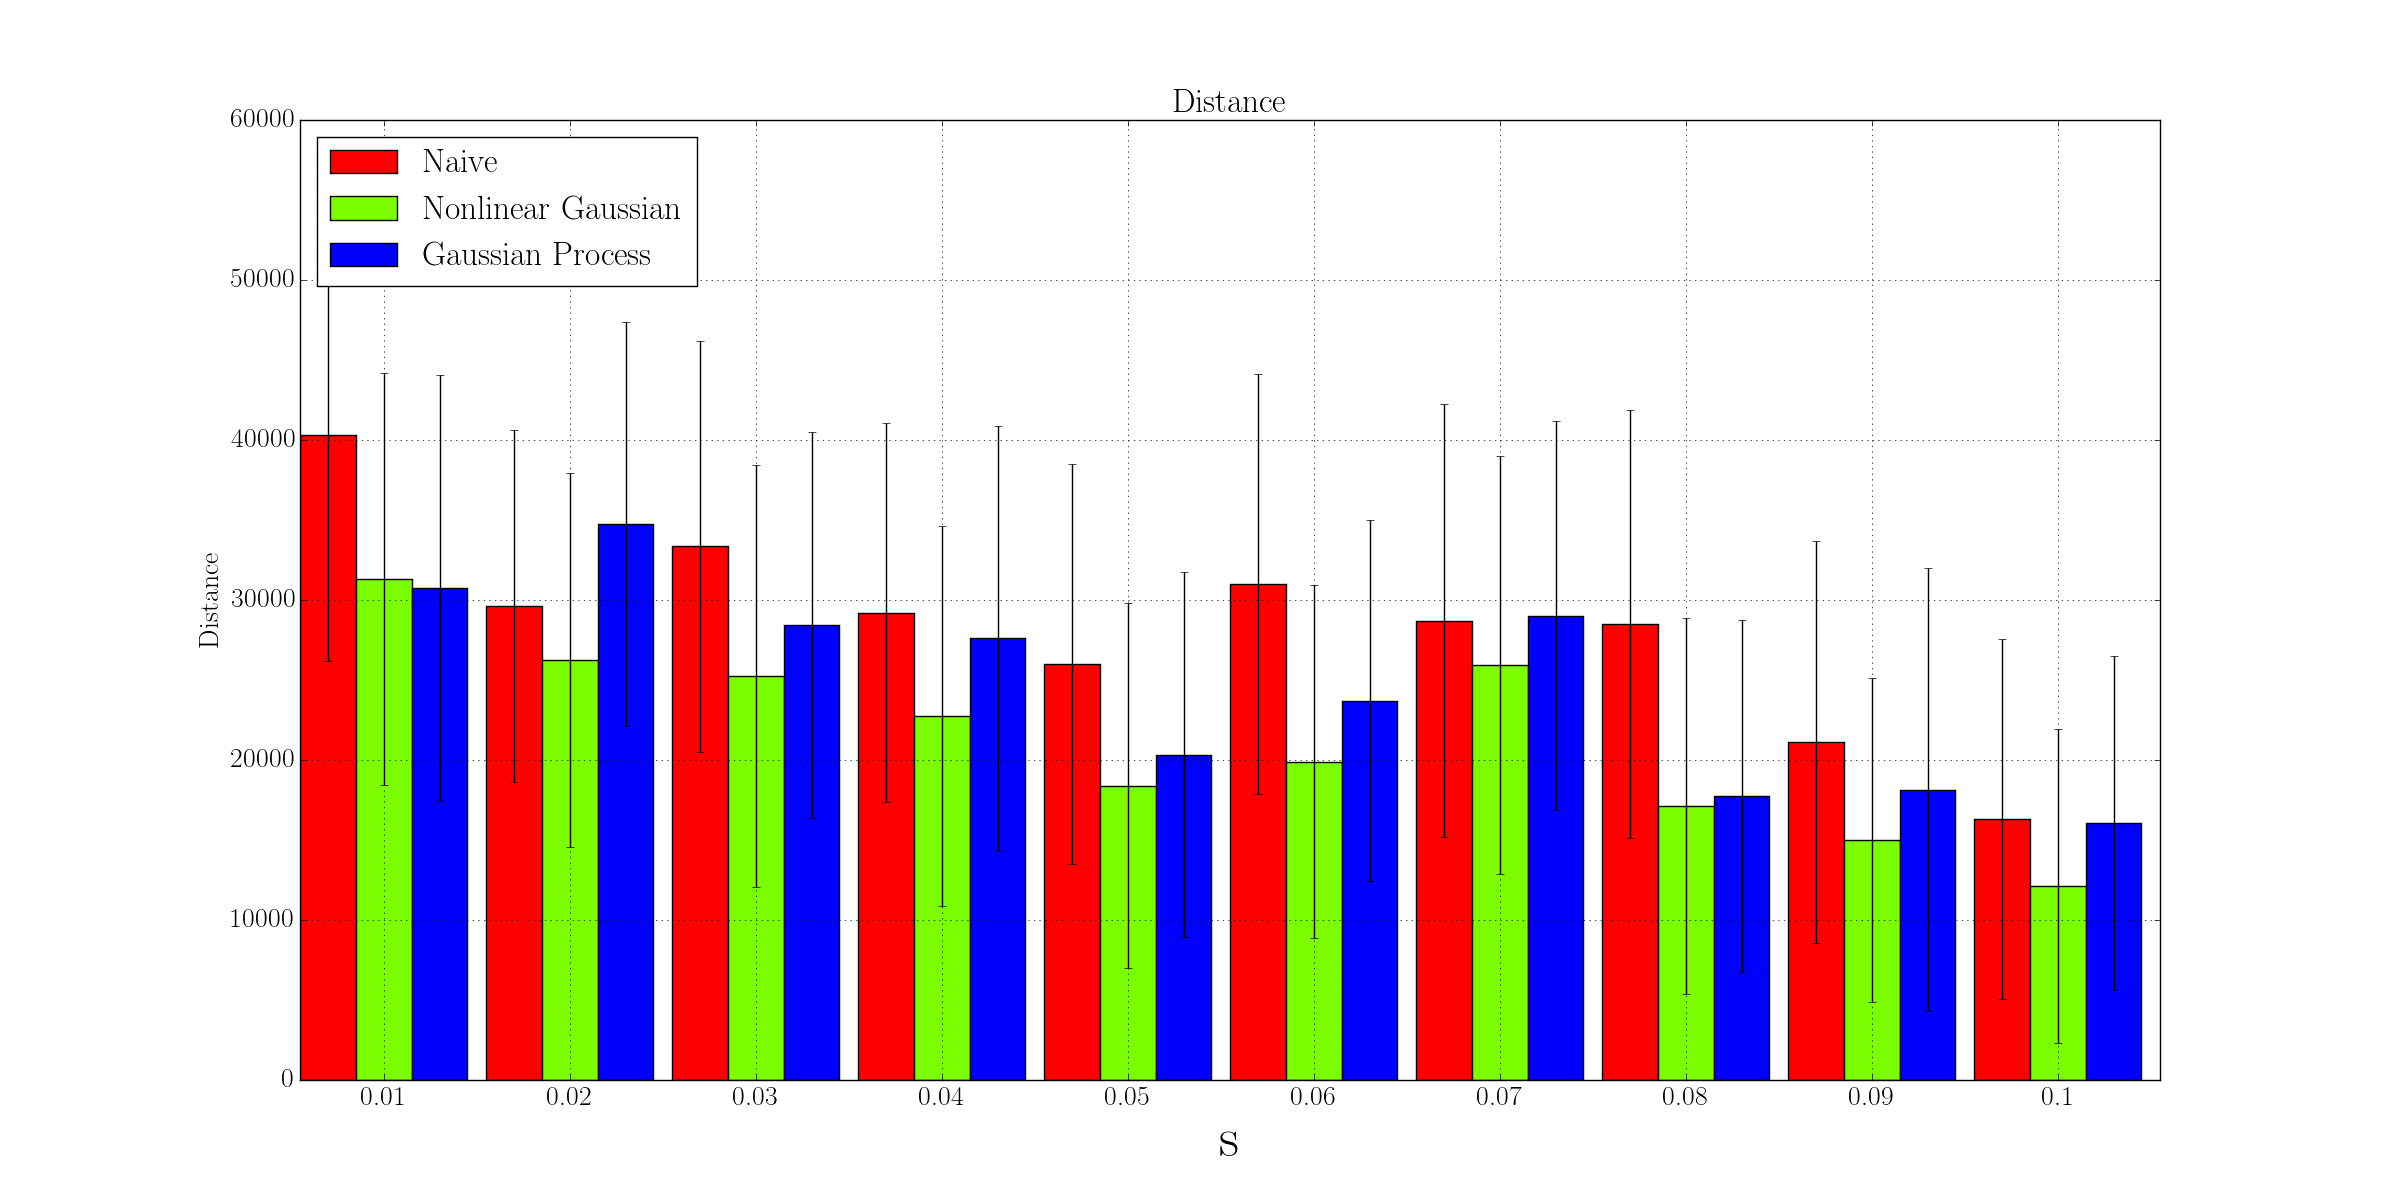
\includegraphics[width=\textwidth]{dist}
\end{figure}
\end{frame}
\begin{frame}{Locating The Site Under Selection: Rank I}
  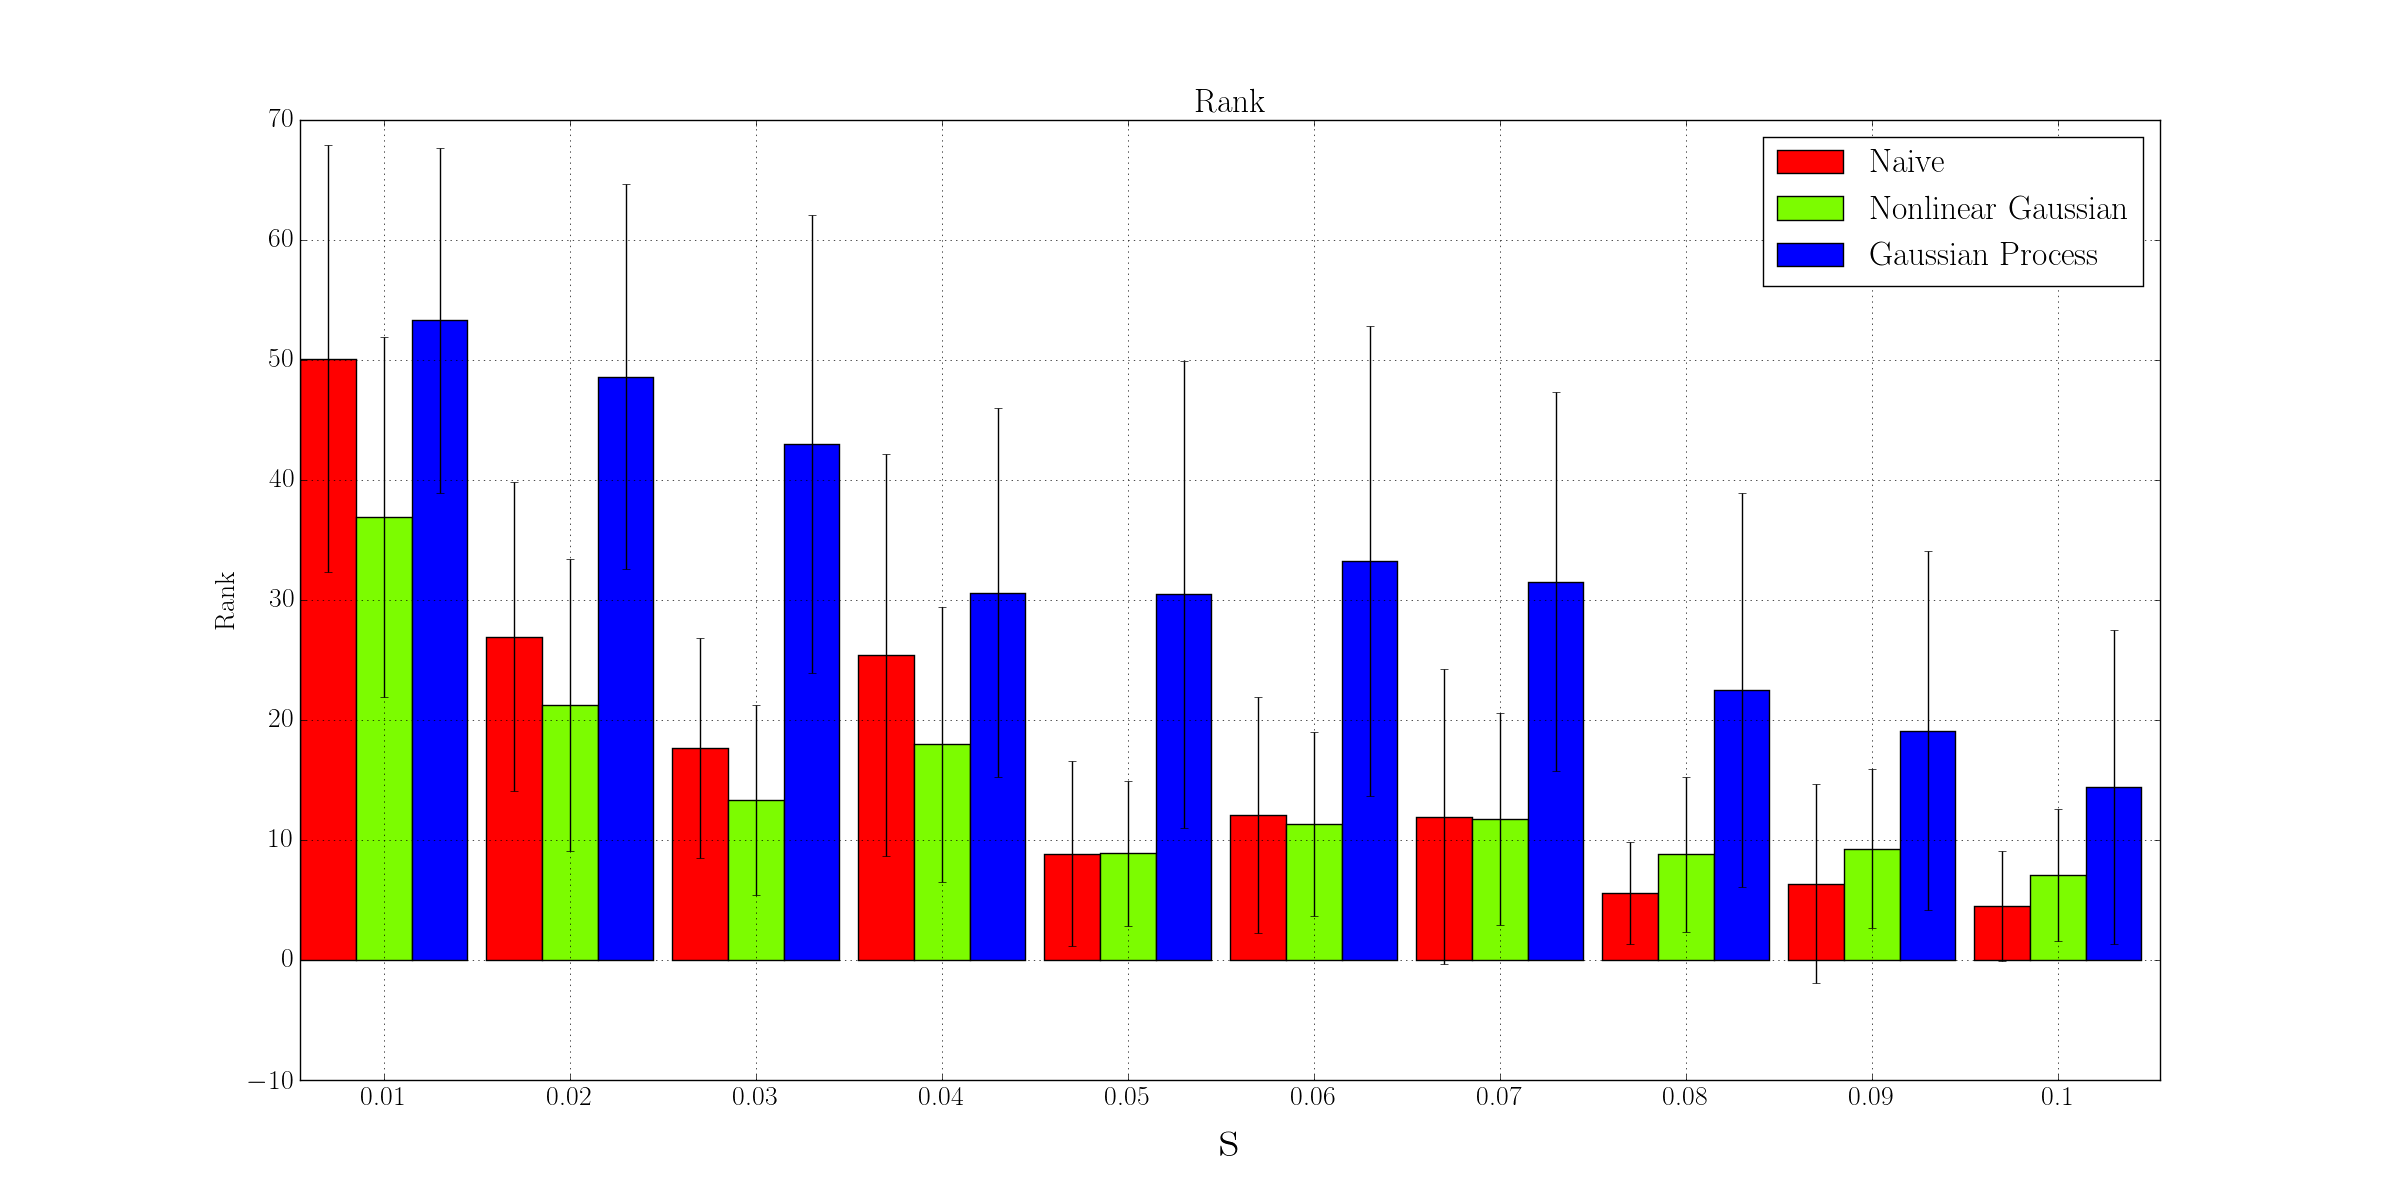
\includegraphics[scale=0.22]{rank}
\end{frame}
\begin{frame}{Locating The Site Under Selection: Rank II}
Mean Reciprocal Rank = 1/Rank of the First Hit
\begin{figure}[H]
  \centering
    \begin{tabular}{c}
  		    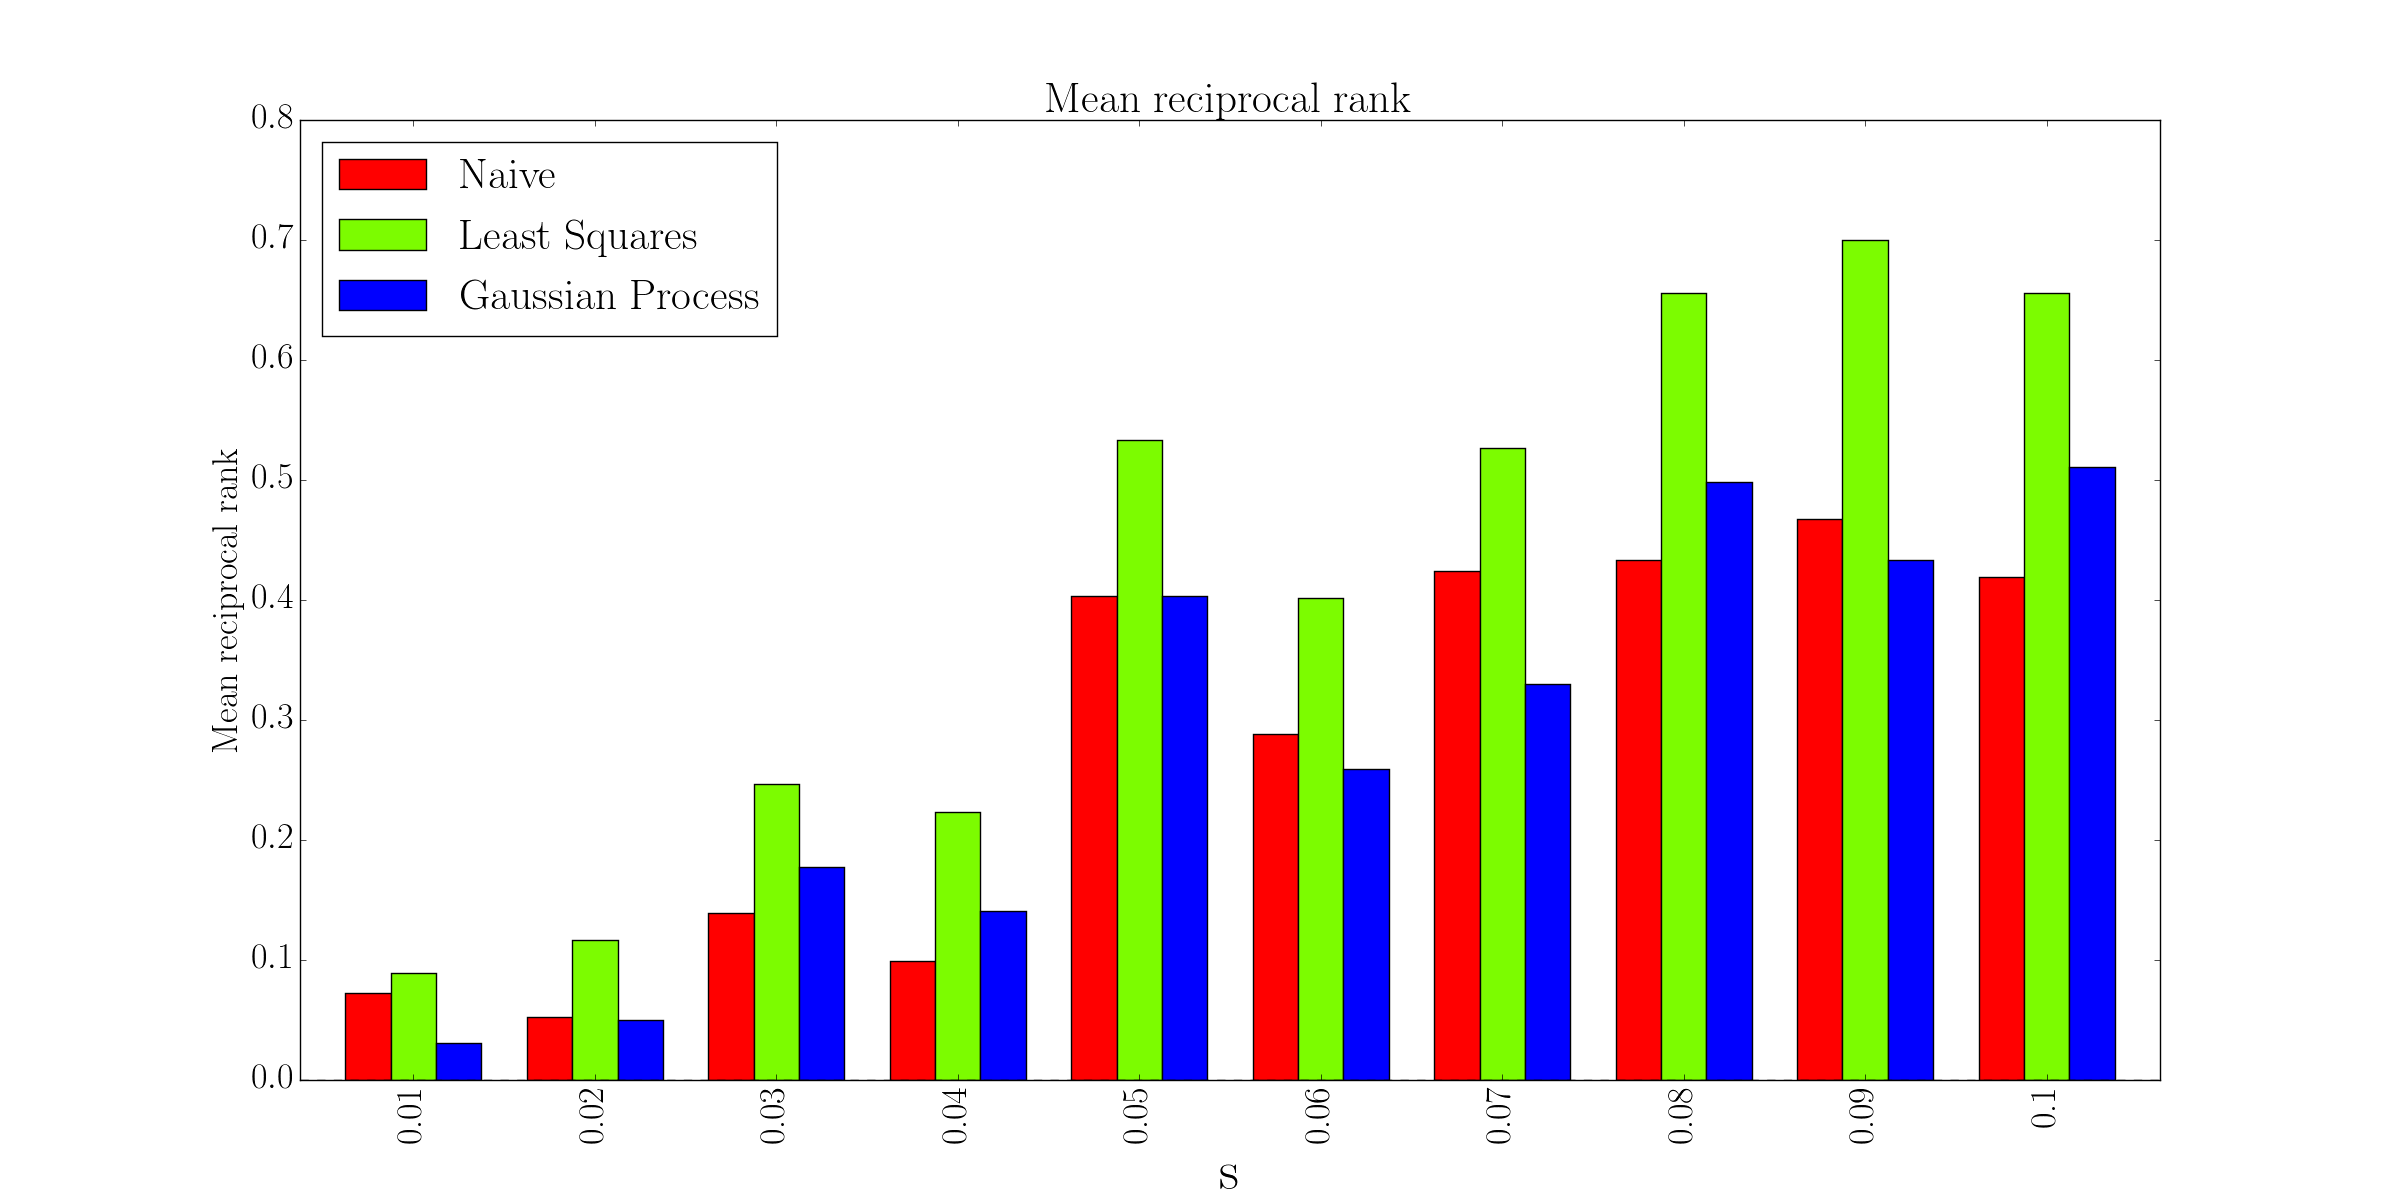
\includegraphics[width=\textwidth]{mrr}
  \end{tabular}
\end{figure}
\end{frame}



\begin{frame}{Computational Performance}
\begin{figure}[H]
  \centering
    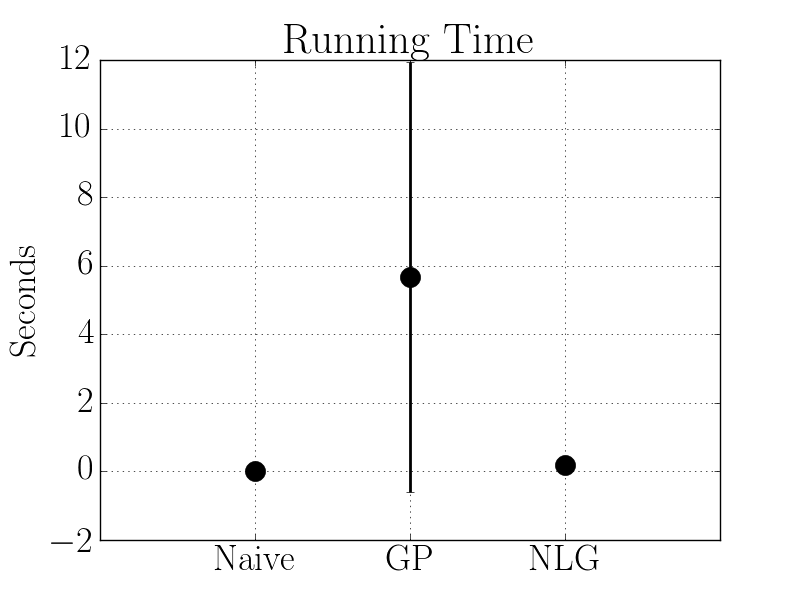
\includegraphics[width=0.6\textwidth]{times}
\end{figure}
\end{frame}





\section{Summary \& Future Work}
\begin{frame}{Summary}
\begin{itemize}
\item We proposed  a Naive method and a nonlinear Gaussian method which outperforms state-of-the-art Gaussian process method on single locus.
\item Performance on the cases with weaker selection is not satisfactory.
\end{itemize}
\end{frame}
\begin{frame}{Future Works}
\begin{enumerate}[I]
\item In addition to low signal-to-noise ratio, fixed sampling through time has led to poor performance in weak selection scenarios. In real world scenario we do not have a priori about strength of selection to set a resolution for sampling.
\begin{itemize}
\item We will address this issue by an adaptive sampling issue. I.e., we decide when to take next sample by observing changes in AF, so far.
\end{itemize}
\item Currently we are using single locus, and the linkage between sites is ignored. 
\begin{itemize}
\item The model is extended by observing multi-locus population statistic. I.e., we aim to estimate the random process of average HAF\footnote{Ronen, Roy, et al. "Haplotype Allele Frequency (HAF) Score: Predicting Carriers of Ongoing Selective Sweeps Without Knowledge of the Adaptive Allele." 2015.} for every sliding window.
\end{itemize}

\end{enumerate}


\end{frame}
\begin{frame}{.}
\vspace{1	in}
\begin{center}
	\huge{Thanks!}\\
		\huge{Questions?}\\
\end{center}

\end{frame}
\end{document}


